\section*{Problem 1 - Attitude Control of Satellite}

\subsection*{Problem 1.1}

The equilibrium point $\boldsymbol{x}_0$ of the closed-loop $\boldsymbol{x} = [ \boldsymbol{\epsilon}^T, \boldsymbol{\omega}^T]^T$ can be found by looking at $\dot{\boldsymbol{q}} = \boldsymbol{0}$ to find $\boldsymbol{\omega}$. 

\begin{align}
\boldsymbol{\dot{q}} &= 
\boldsymbol{T}_q(\boldsymbol{q})\boldsymbol{\omega}\\ 
&= \frac{1}{2}
\begin{bmatrix}
-\epsilon_1 & -\epsilon_2 & -\epsilon_3 \\
\eta & -\epsilon_3 & \epsilon_2 \\
\epsilon_3 & \eta & \epsilon_1 \\
-\epsilon_2 & \epsilon_1 & \eta 
\end{bmatrix}
\boldsymbol{\omega} \\
&= \frac{1}{2}
\begin{bmatrix}
0 & 0 & 0 \\
1 & 0 & 0 \\
0 & 1 & 0 \\
0 & 0 & 1
\end{bmatrix}
\boldsymbol{\omega} = \boldsymbol{0} \\
\end{align}
This gives \\
\begin{align}
   \boldsymbol{\omega}= 
   \begin{bmatrix}
   0 & 0 & 0
   \end{bmatrix}
\end{align}

Therefore, when $\boldsymbol{\epsilon}=[0 , 0 , 0]^T$ we have \\
\begin{align}
    \boldsymbol{x}_0 =
    \begin{bmatrix}
    \boldsymbol{\epsilon}^T \\
    \boldsymbol{\omega}^T
    \end{bmatrix}
    = 
    \begin{bmatrix}
    0 \\
    0 \\
    0 \\
    0 \\
    0 \\
    0
    \end{bmatrix}
\end{align}

Linearizing about $\boldsymbol{x} = \boldsymbol{x}_0$ gives
\begin{align}
    \boldsymbol{I}_{CG}\boldsymbol{\dot{\omega}} &= \boldsymbol{S}(\boldsymbol{I}_{CG}\boldsymbol{\omega})\boldsymbol{\omega} + \boldsymbol{\tau}  \\
    \boldsymbol{\dot{\omega}} &= \boldsymbol{I}^{-1}_{CG}\boldsymbol{S}(\boldsymbol{I}_{CG}\boldsymbol{\omega})\boldsymbol{\omega} + \boldsymbol{I}^{-1}_{CG}\boldsymbol{\tau} \\
\end{align}
and
\begin{align}
    \boldsymbol{\dot{x}} &= 
    \begin{bmatrix}
    \boldsymbol{\dot{\epsilon}}^T \\
    \boldsymbol{\dot{\omega}}^T
    \end{bmatrix}
    =
    \begin{bmatrix}
    \frac{1}{2}\boldsymbol{\omega^T} \\
    \boldsymbol{I}^{-1}_{CG}\boldsymbol{S}(\boldsymbol{I}_{CG}\boldsymbol{\omega})\boldsymbol{\omega} + \boldsymbol{I}^{-1}_{CG}\boldsymbol{\tau}
    \end{bmatrix}
    = \mathbf{h}(\mathbf{x},\mathbf{u}) \\
\end{align}
Where we have
\begin{align}
    \boldsymbol{I}^{-1}_{CG}\boldsymbol{S}(\boldsymbol{I}_{CG}\boldsymbol{\omega})\boldsymbol{\omega} &= 
    \frac{1}{mr^2} 
    \begin{bmatrix}
    1 & 0 & 0 \\
    0 & 1 & 0 \\
    0 & 0 & 1 \\
    \end{bmatrix}
    \begin{bmatrix}
     0 & -mr^2\omega & mr^2\omega \\
     mr^2\omega & 0 & -mr^2\omega \\
     -mr^2\omega & mr^2\omega & 0 \\
    \end{bmatrix} \\
    &= 
    \begin{bmatrix}
    0 & 0 & 0 \\
    0 & 0 & 0 \\
    0 & 0 & 0 
    \end{bmatrix}
\end{align}

We then linearize:
\begin{equation}
    \mathbf{A} = \frac{\delta \mathbf{h(x,u)}}{\delta \mathbf{x}} |_{\mathbf{x^*, u^*}}, 
    \quad \mathbf{B} = \frac{\delta \mathbf{h(x,u)}}{\delta \mathbf{u}} |_{\mathbf{x^*, u^*}}, \\
\end{equation}



This gives A matrix
\begin{align}
    \boldsymbol{A} = 
    \begin{bmatrix}
    0 & 0 & 0 & \frac{1}{2} & 0 & 0 \\
    0 & 0 & 0 & 0 & \frac{1}{2} & 0 \\
    0 & 0 & 0 & 0 & 0 & \frac{1}{2} \\
    0 & 0 & 0 & 0 & 0 & 0 \\
    0 & 0 & 0 & 0 & 0 & 0 \\
    0 & 0 & 0 & 0 & 0 & 0 
    \end{bmatrix}
\end{align}
And B matrix given by the second part of $\boldsymbol{\dot{\omega}}$ 
\begin{align}
\boldsymbol{B} = 
\begin{bmatrix}
    0 & 0 & 0 \\
    0 & 0 & 0 \\
    0 & 0 & 0 \\
    \frac{1}{mr^2} & 0 & 0 \\
    0 & \frac{1}{mr^2} & 0 \\
    0 & 0 & \frac{1}{mr^2} 
\end{bmatrix}
\end{align}

\subsection*{Problem 1.2}

With our state space expression from 1.2 and $\boldsymbol{\tau} = -\boldsymbol{K}_d\boldsymbol{\omega} - k_p\boldsymbol{\epsilon}$ we have
\begin{align}
    \boldsymbol{\dot{x}} = \boldsymbol{A}\boldsymbol{x} + \boldsymbol{B}(-\boldsymbol{K}_d\boldsymbol{\omega} - k_p\boldsymbol{\epsilon})
\end{align}
This gives
\begin{align}
    \boldsymbol{\dot{x}} = 
    \begin{bmatrix}
    0 & 0 & 0 & \frac{1}{2} & 0 & 0 \\
    0 & 0 & 0 & 0 & \frac{1}{2} & 0 \\
    0 & 0 & 0 & 0 & 0 & \frac{1}{2} \\
    -\frac{k_p}{mr^2} & 0 & 0 & -\frac{k_d}{mr^2} & 0 & 0 \\
    0 & -\frac{k_p}{mr^2} & 0 & 0 & -\frac{k_d}{mr^2} & 0 \\
    0 & 0 & -\frac{k_p}{mr^2} & 0 & 0 & -\frac{k_d}{mr^2}
    \end{bmatrix}
\end{align}

Inserted into MATLAB we calculate the eigenvalues to be complex, all in the left half plane. The eigenvalues in the linearized system are therefore stable.

In this particular application we would like to have our poles result in a critically damped response, $\zeta = 1$, given by poles with negative real part and no complex part\cite{regtek}. However, whether the poles are real or complex does not matter too much because the system is linearized meaning that the system response will not be accurate to the real system response anyway. Any inaccuracies in modeling will alter the damping ratio of the actual system. 

\subsection*{Problem 1.3}

Simulating with the given initial conditions gives the plots in Figure \ref{fig:onethree}. The system response seems reasonable, all angles and velocities reach their desired reference of zero, and the control input approaches zero. This seems reasonable as the system is not affected by any external disturbances. We introduce a reference by changing the control law to equation \ref{eq:nonzeroCL}, this allows us to follow nonzero references.

\begin{align}\label{eq:nonzeroCL}
    \boldsymbol{\tau} = \boldsymbol{K}_d(\boldsymbol{\omega}_r -\boldsymbol{\omega}) + k_p(\boldsymbol{\epsilon}_r -\boldsymbol{\epsilon})
\end{align}


\begin{figure}[h]
    \centering
    \begin{subfigure}[b]{0.45\textwidth}
        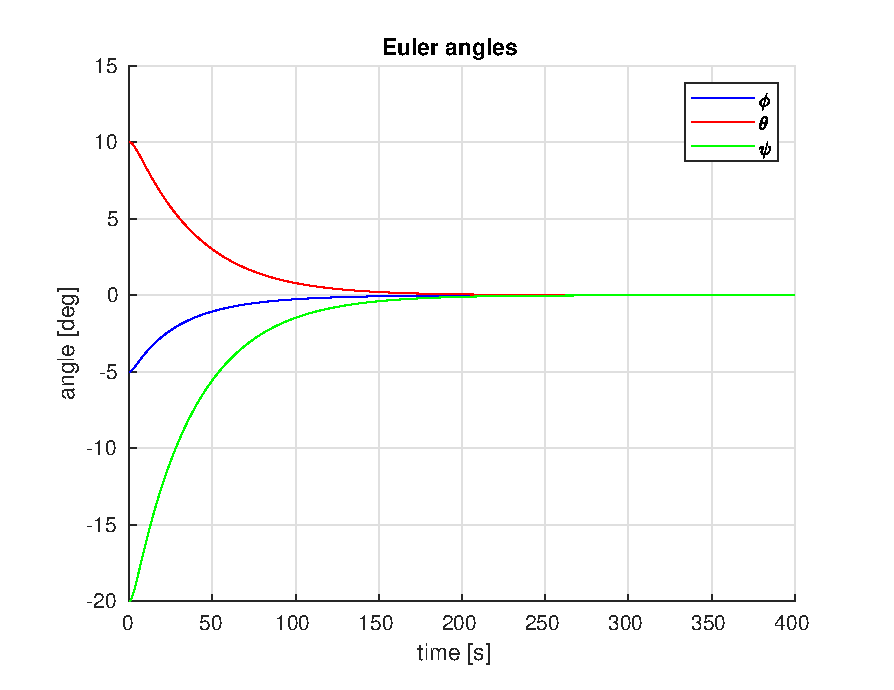
\includegraphics[width=\textwidth]{plots/euler_angles_13.eps}
        \caption{Euler Angles}
        \label{fig:euler}
    \end{subfigure}
    \begin{subfigure}[b]{0.45\textwidth}
        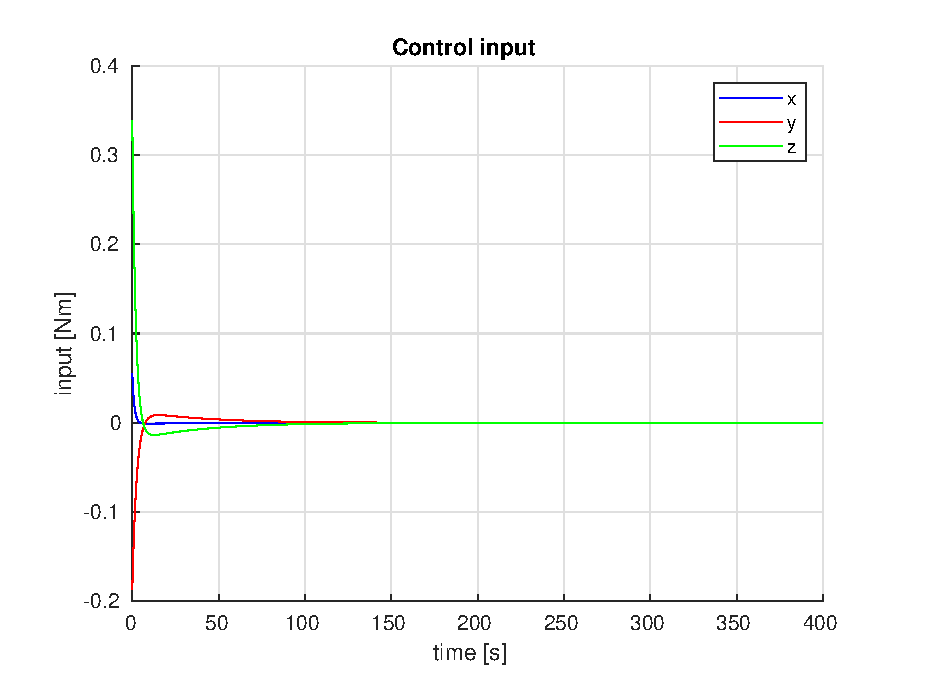
\includegraphics[width=\textwidth]{plots/control_input_13.eps}
        \caption{Control Input}
        \label{fig:input}
    \end{subfigure}
    \begin{subfigure}[b]{0.45\textwidth}
        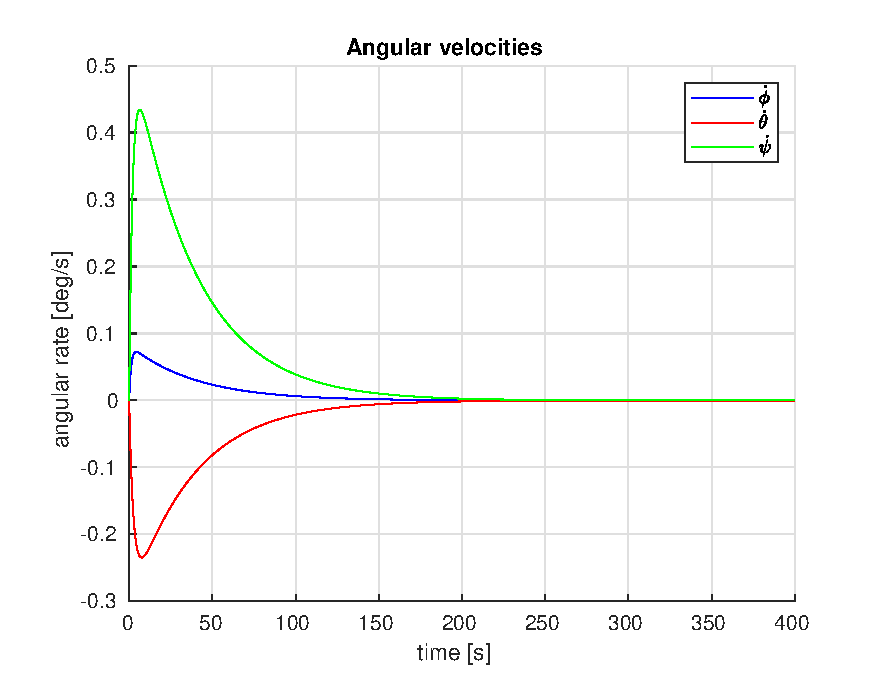
\includegraphics[width=\textwidth]{plots/angular_velocities_13.eps}
        \caption{Angular Velocities}
        \label{fig:angular}
    \end{subfigure}
    \caption{Simulation of attitude dynamics}\label{fig:onethree}
\end{figure}


\subsection*{Problem 1.4}
The quaternion error can be written as
 \begin{equation}
	 \tilde{\mathbf{q}} := \left[
	 \begin{array}{c}
		 \tilde{\eta} \\
		 \tilde{\epsilon}
	 \end{array}
	 \right] = \bar{\mathbf{q}}_d \otimes \mathbf{q} 
 \end{equation}
 
 Because we have 
 \begin{align}
     \bar{\boldsymbol{q}} = 
     \begin{bmatrix}
         \boldsymbol{\eta} \\
         -\boldsymbol{\epsilon}^T
     \end{bmatrix}
 \end{align}
 and
 \begin{align}
     \boldsymbol{q} = 
     \begin{bmatrix}
         {\eta} \\
         {\epsilon}^T
     \end{bmatrix}
 \end{align}
 We get
 \begin{align}
     \boldsymbol{\tilde{q}} = 
     \begin{bmatrix}
         \eta_d\eta + \epsilon_d^T\epsilon \\
         \eta_d\epsilon - \eta\epsilon_d - S(\epsilon_d)\epsilon
     \end{bmatrix}
 \end{align}
 
 We find $S(\epsilon_d)\epsilon$ to be
 \begin{align}
     S(\epsilon_d)\epsilon = 
     \begin{bmatrix}
         0 & -\epsilon_{3,d} & \epsilon_{2,d} \\
         \epsilon_{3,d} & 0 & -\epsilon_{1,d} \\
         -\epsilon_{2,d} & \epsilon_{1,d} & 0 
     \end{bmatrix}
     \begin{bmatrix}
         \epsilon_1 \\
         \epsilon_2 \\
         \epsilon_3
     \end{bmatrix}
     = 
    \begin{bmatrix}
        -\epsilon_{3,d}\epsilon_{2} + \epsilon_{2,d}\epsilon_{3} \\
        \epsilon_{3,d}\epsilon_{1} - \epsilon_{1,d}\epsilon_{3} \\
        -\epsilon_{2,d}\epsilon_{1} + \epsilon_{1,d}\epsilon_{2}
    \end{bmatrix}
 \end{align}

Which when $q=q_d$ yields 
\begin{align}
    \boldsymbol{\tilde{q}} = 
    \begin{bmatrix}
        \eta^2 + \epsilon^2 \\
        -\epsilon_{3}\epsilon_{2} + \epsilon_{2}\epsilon_{3} \\
        \epsilon_{3}\epsilon_{1} -\epsilon_{1}\epsilon_{3} \\
        -\epsilon_{2}\epsilon_{1} + \epsilon_{1}\epsilon_{2}
    \end{bmatrix}
    = 
    \begin{bmatrix}
       1- \epsilon^2+ \epsilon^2 \\
        0 \\
        0 \\
        0
    \end{bmatrix}
    =
    \begin{bmatrix}
        1 \\
        0 \\
        0 \\
        0
    \end{bmatrix}
\end{align}
\subsection*{Problem 1.5}
Simulating the attitude dynamics with the given parameters we get the plots in Figure \ref{fig:onefive}. We can see that $\phi$ goes to approximately zero and $\theta$ and $\psi$ is approximating cosine and sine but a large reference tracking error. 

Figure \ref{fig:trackerr} shows the tracking error. We penalize any nonzero $\omega$ in our control law, while trying to follow a nonzero reference. This leads to a very damped system response and the large tracking error that we observe.

\begin{figure}[h]
    \centering
    \begin{subfigure}[b]{0.45\textwidth}
        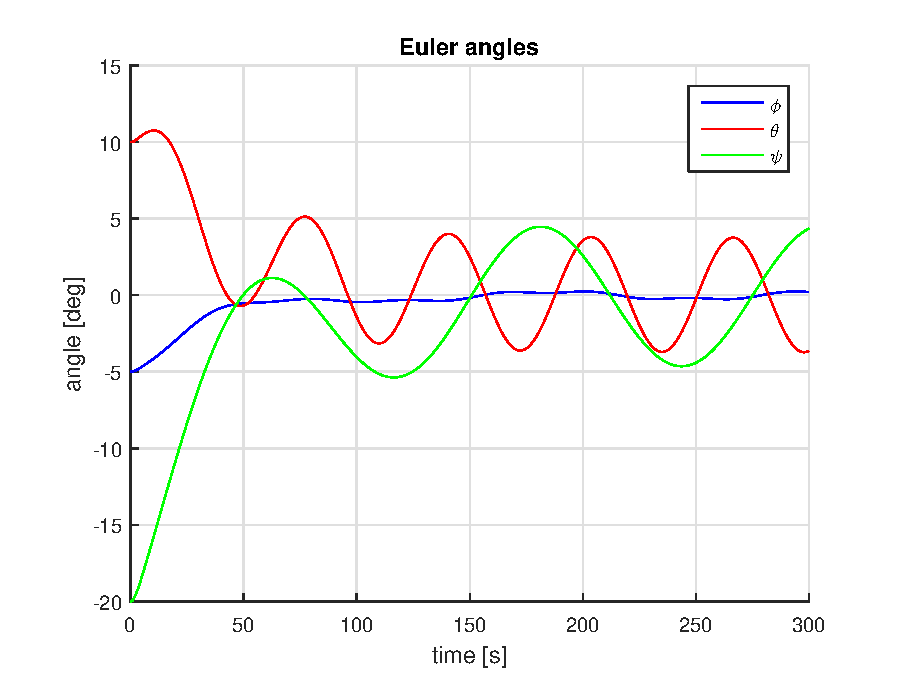
\includegraphics[width=\textwidth]{plots/euler_angles_155.eps}
        \caption{Euler Angles}
        \label{fig:euler5}
    \end{subfigure}
    \begin{subfigure}[b]{0.45\textwidth}
        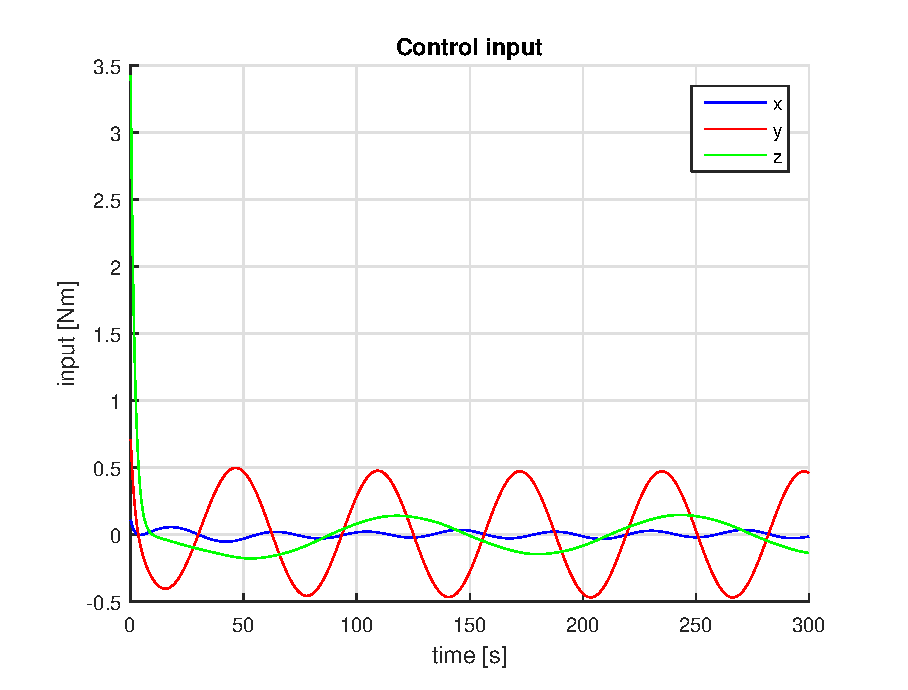
\includegraphics[width=\textwidth]{plots/control_input_155.eps}
        \caption{Control Input}
        \label{fig:input5}
    \end{subfigure}
    \begin{subfigure}[b]{0.45\textwidth}
        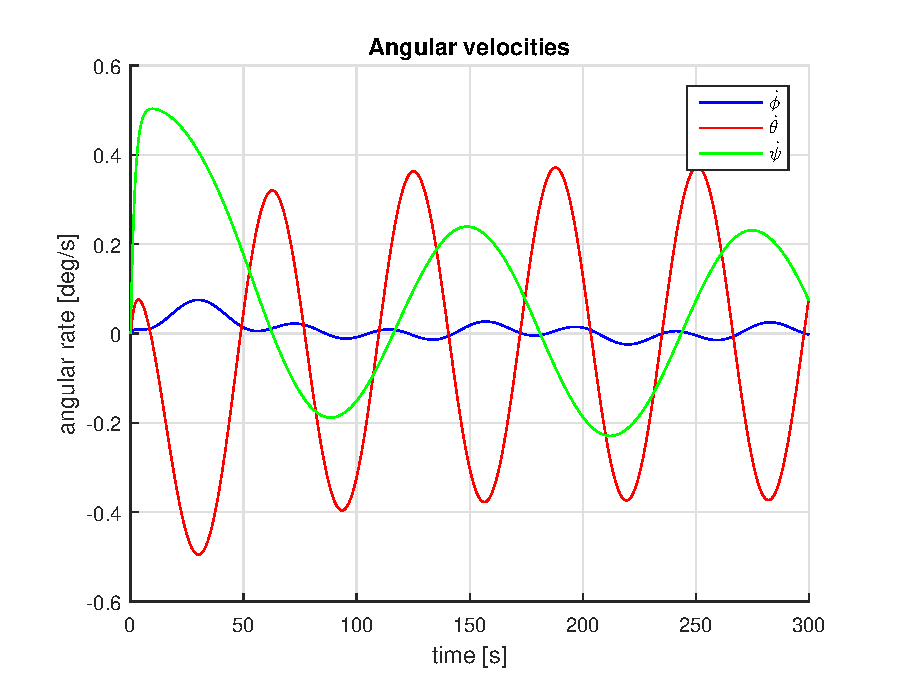
\includegraphics[width=\textwidth]{plots/angular_velocities_155.eps}
        \caption{Angular Velocities}
        \label{fig:angular5}
    \end{subfigure}
    \caption{Simulation of attitude dynamics}\label{fig:onefive}
\end{figure}


\begin{figure}[h]
    \centering
    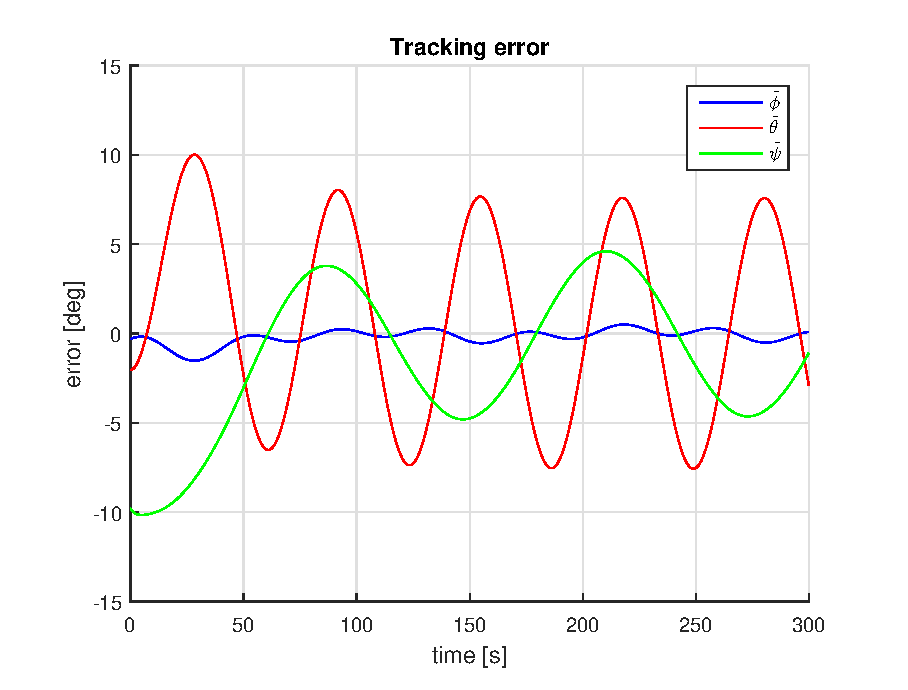
\includegraphics{plots/tracking_error_15.eps}
    \caption{Tracking Error}
    \label{fig:trackerr}
\end{figure}



\subsection*{Problem 1.6}
The control law in this problem can be written as
\begin{equation}
	\boldsymbol{\tau} = -\mathbf{K}_d \tilde{\boldsymbol{\omega}} - k_p \tilde{\boldsymbol{\epsilon}}
\end{equation}
and the desired angular velocity as
\begin{equation}
	\boldsymbol{\omega}_d = \mathbf{T}^{-1}_{\Theta_d}(\Theta_d)\dot{\Theta}_d
\end{equation}

We have: \\
\begin{align}
    {\phi}(t) &= 0 \\
    {\theta}(t) &= 15\cos(0.1t) \\
    {\psi}(t) &= 10\sin(0.05t) \\
    \dot{\phi}(t) &= 0 \\
    \dot{\theta}(t) &= -1.5\sin(0.1t) \\
    \dot{\psi}(t) &= 0.5\cos(0.05t)
\end{align}

Which gives

\begin{align}
\boldsymbol{\omega}_d &= \boldsymbol{T}^{-1}_{\Theta_d}(\boldsymbol{\Theta}_d) \\ 
&= 
\begin{bmatrix}
    1 & 0 & -\sin(\theta_d) \\
    0 & \cos(\phi_d) & \cos(\theta_d)\sin(\phi_d) \\
    0 & -\sin(\phi_d) & \cos(\theta_d)\cos(\phi_d) \\
\end{bmatrix}
\begin{bmatrix}
    0 \\
    -1.5\sin(0.1t) \\
    0.5\cos(0.05t)
\end{bmatrix} \\
\Rightarrow &= 
\begin{bmatrix}
    -0.5\sin(\theta_d)\cos(0.05t) \\
    - 1.5\sin(0.1t)\cos(\phi_d) + 0.5\cos(0.05t)\cos(\theta_d)\sin(\phi_d) \\
    1.5\sin(\phi_d)\sin(0.1t) +0.5\cos(0.05t)\cos(\theta_d)\cos(\phi_d)
\end{bmatrix}
\end{align}

\begin{figure}[h]
    \centering
    \begin{subfigure}[b]{0.45\textwidth}
        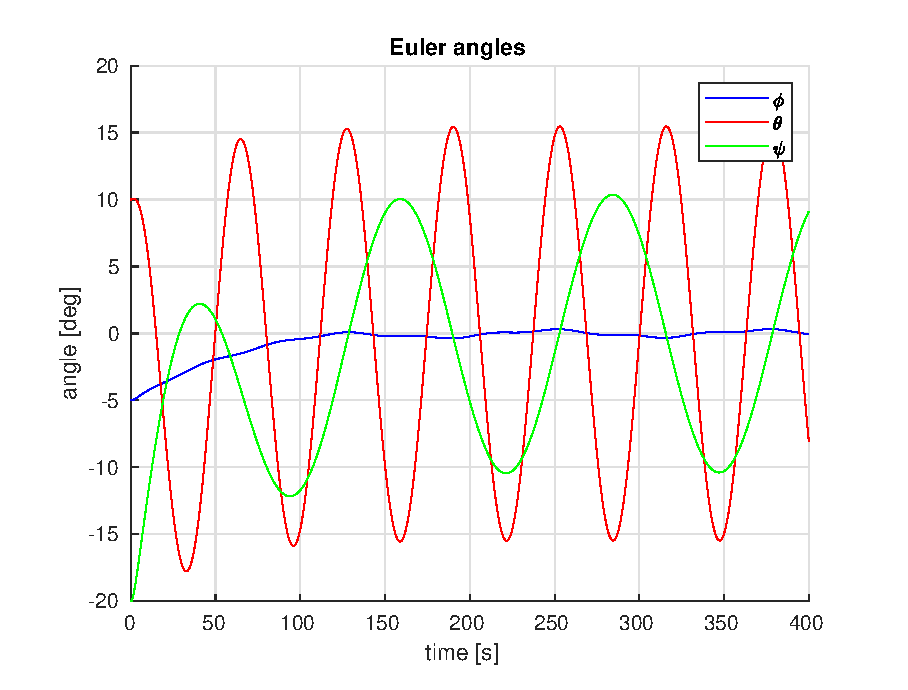
\includegraphics[width=\textwidth]{plots/euler_angles_16.eps}
        \caption{Euler Angles}
        \label{fig:euler6}
    \end{subfigure}
    \begin{subfigure}[b]{0.45\textwidth}
        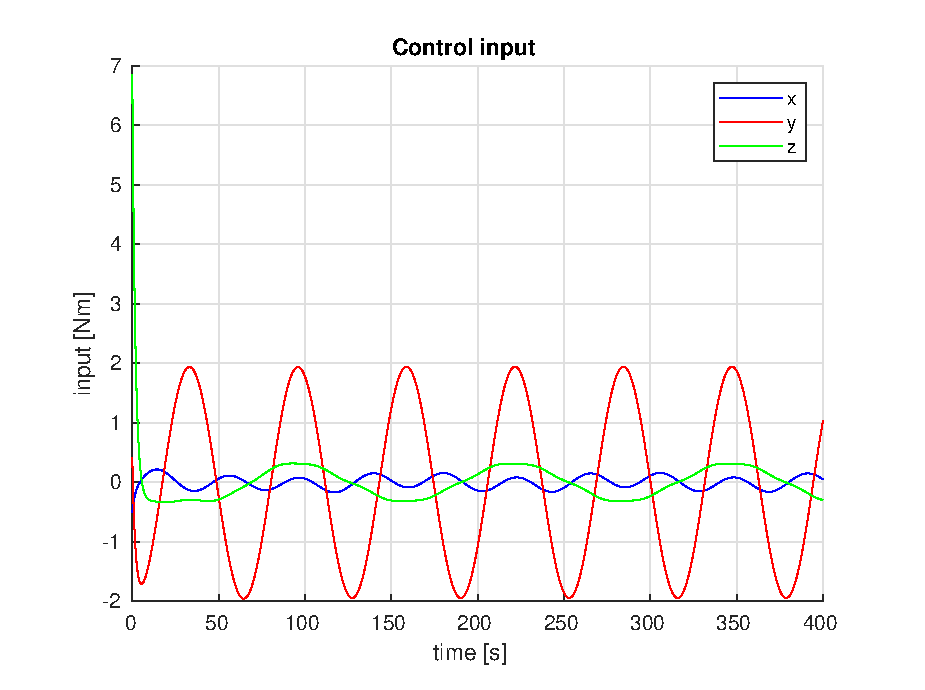
\includegraphics[width=\textwidth]{plots/control_input_16.eps}
        \caption{Control Input}
        \label{fig:input6}
    \end{subfigure}
    \begin{subfigure}[b]{0.45\textwidth}
        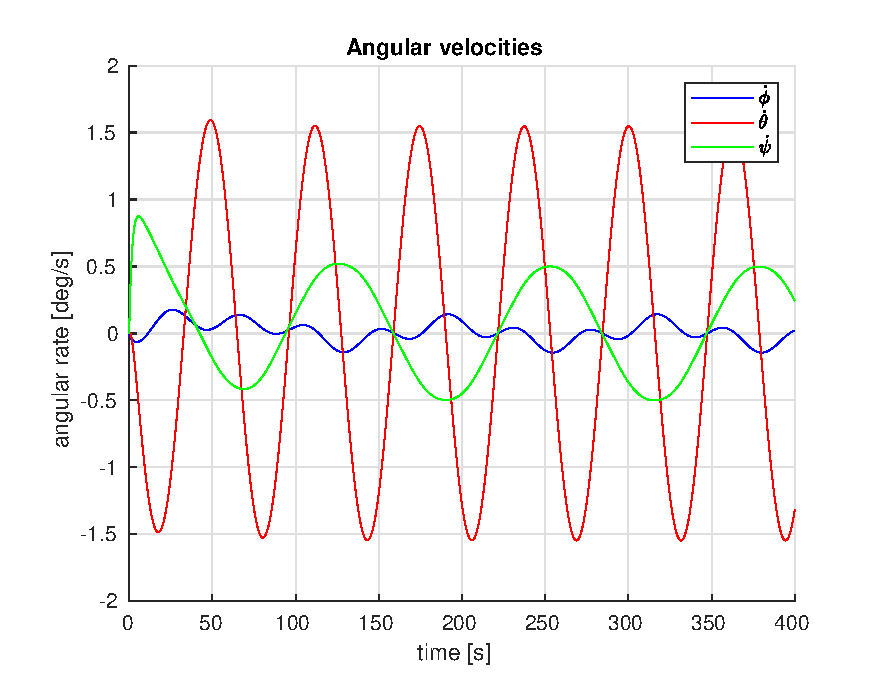
\includegraphics[width=\textwidth]{plots/angular_velocities_16.eps}
        \caption{Angular Velocities}
        \label{fig:angular6}
    \end{subfigure}
    \caption{Simulation of attitude dynamics}\label{fig:onesix}
\end{figure}

\begin{figure}[h]
    \centering
    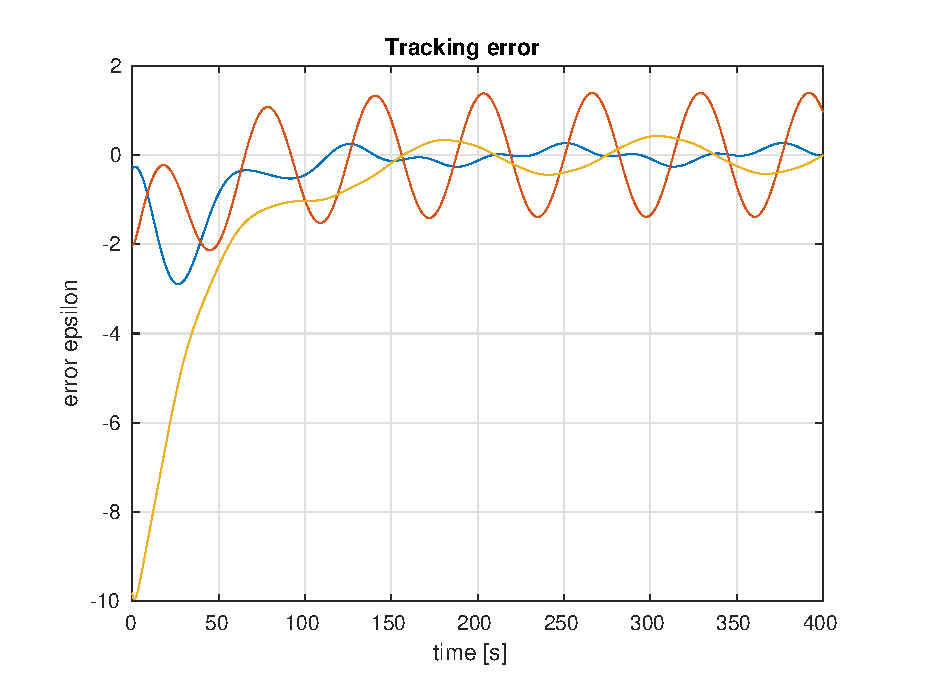
\includegraphics{plots/tracking_error_16.eps}
    \caption{Tracking Error}
    \label{fig:trackerr2}
\end{figure}

By looking at the simulation plots in Figure \ref{fig:onesix} we can see that $\theta$ and $\psi$ now actually follow the reference and $\phi$ is a little bit better than the previous task. This can be confirmed by looking at the tracking error, figure \ref{fig:trackerr2}, which is significantly better than the previous task, and is caused by the change from $\omega$ to $\tilde{\omega}$ in the control law. \\
A way to further improve this result can be to add an integral term or to find a control law with a candidate function which gives a negative definite derivation such that the equilibrium is globally exponentially stable\cite{Khalil}. \\

\subsection*{Problem 1.7}
The Lyapunov function can be written as 
 \begin{equation}
	 V = \frac{1}{2} \tilde{\boldsymbol{\omega}}^{\top} \mathbf{I}_{CG}\tilde{\boldsymbol{\omega}} + 2 k_p (1-\tilde{\eta})
 \end{equation}

We want to prove that V is positive:
\begin{align}
    \bf{I}_{CG} &> 0 \\
    \Rightarrow \tilde{\bf{\omega}}\bf{I}_{CG}\tilde{\bf{\omega}}&>0 \\
    k_p &> 0 \\ 
    \tilde{\bf{\omega}} &= \bf{\omega} - \bf{\omega_d} = \bf{\omega} \\
\end{align}

$\tilde{\bf{\eta}}$ is a quaternion and thus $\tilde{\bf{\eta}}\leq 1 \Rightarrow (1-\tilde{\bf{\eta}}) \geq 0 $. As such, V is positive. \\

We then also see that \\
\begin{align}
    \lim_{\omega \rightarrow \infty}V = \infty
\end{align}

We then want to show that
\begin{align}
    \dot{V} = -k_d\omega^T\omega
\end{align}
\begin{align}
     V = \frac{1}{2} \tilde{\boldsymbol{\omega}}^{\top} \mathbf{I}_{CG}\tilde{\boldsymbol{\omega}} + 2 k_p (1-\tilde{\eta}) \\
     I_{CG}\dot{\omega} - S(I_{CG}\omega)\omega = \tau \\
     \Rightarrow \dot{\omega} = \frac{\tau + \omega S(I_{CG}\omega)}{I_{CG}} \\
     \dot{\tilde{\eta}} = -\frac{1}{2}\tilde{\epsilon}^T\tilde{\omega} \\
     \tau = -K_d\omega - k_p\tilde{\epsilon} \\
\end{align}

\begin{align} \label{equation}
     S(I_{CG}\omega)\omega &=
     \begin{bmatrix}
         0 & -mr^2\omega_3 & mr^2\omega_2 \\
         mr^2\omega_3 & 0 & -mr^2\omega_1 \\
         -mr^2\omega_2 & mr^2\omega_1 & 0 
     \end{bmatrix}
     \begin{bmatrix}
         \omega_1 \\
         \omega_2 \\
         \omega_3 
     \end{bmatrix} \\
     &= 
     \begin{bmatrix}
         -mr^2\omega_3\omega_2 + mr^2\omega_2\omega_3 \\
         mr^2\omega_3\omega_1 - mr^2\omega_1\omega_3 \\
         -mr^2\omega_2\omega_1 + mr^2\omega_1\omega_2 
     \end{bmatrix} \\
     &= 
     \begin{bmatrix}
         0 \\
         0 \\
         0
     \end{bmatrix} 
\end{align}

Which with the use of (\ref{equation}) gives 
\begin{align}
    \dot{V} &= \omega^TI_{CG}\dot{\omega} - 2k_p\dot{\tilde{\eta}} \\
    &= \omega^T(\tau + S(I_{CG}\omega)\omega) + k_p\tilde{\epsilon}^T\tilde{\omega} \\
    &= \omega^T(-K_d\omega - k_p\tilde{\epsilon} +S(I_{CG}\omega)\omega) + k_p\tilde{\epsilon}^T\tilde{\omega} \\
    &= \omega ^T (-K_d\omega) + \omega^TS(I_{CG} \omega)\omega \\
    \Rightarrow \dot{V} &= -k_d\omega^T\omega 
\end{align}

All criteria of Theorem 4.2 in Khalil\cite{Khalil} are satisfied, meaning the equilibrium is globally asymptotically stable.
